In this the Stokes equations are not solved. It is a 2D implementation of the cvi algorithm 
as introduced in \cite{waav15} which deals with the advection of markers. 
$Q_1$ and $Q_2$ basis functions are
used and in both cases the cvi algorithm can be toggled on/off. 
Markers can be distributed regularly or randomly at startup.

Three velocity fields are prescribed on the mesh:
\begin{itemize}
\item the so-called Couette flow of \cite{waav15} 
\item the SolCx solution \cite{XX}
\item a flow created by means of a stream line function (see fieldstone 32)
\end{itemize}

%%%%%%%%%%%%%%%%%%%%%%%%%%%%%%%5
\subsection{Couette flow}

%%%%%%%%%%%%%%%%%%%%%%%%%%%%%%%5
\subsection{SolCx}

%%%%%%%%%%%%%%%%%%%%%%%%%%%%%%%5
\subsection{Streamline flow}

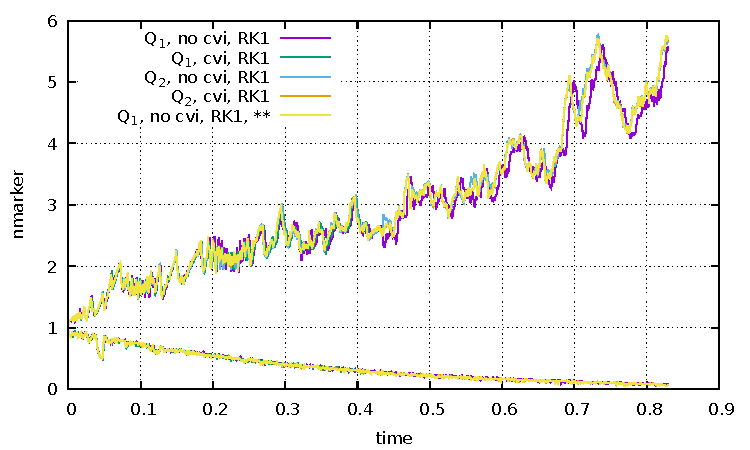
\includegraphics[width=8cm]{python_codes/fieldstone_30/results_streamline/markercount_rk1}
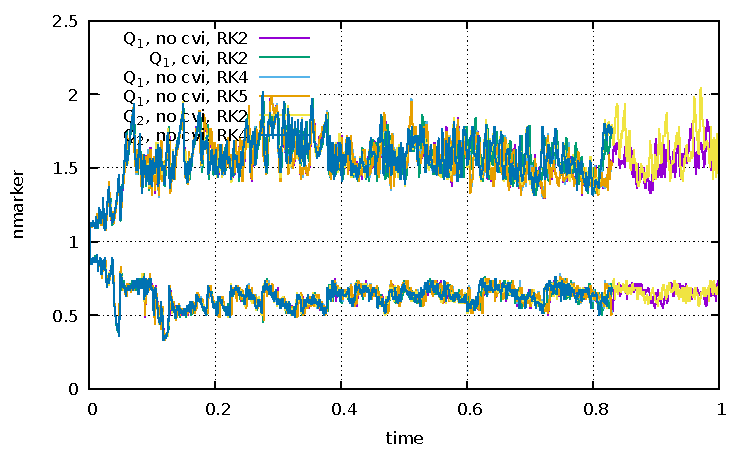
\includegraphics[width=8cm]{python_codes/fieldstone_30/results_streamline/markercount_rk2345}

In this case RK order seems to be more important that cvi. 

Explore why ?! 



\fbox{
\parbox{10cm}{{\bf features}
\begin{itemize}
\item $Q_1\times P_0$ element \index{$Q_1 \times P_0$}
\item incompressible flow \index{incompressible flow}
\item penalty formulation \index{penalty formulation}
\item Dirichlet boundary conditions (free-slip)
\item direct solver 
\item isothermal \index{isothermal}
\item non-isoviscous \index{non-isoviscous}
\item analytical solution \index{analytical solution}
\end{itemize}
}}





